\section{Vista de Implementación} \label{vistaImplementacion}
En esta sección se muestra una abstracción de la interacción de los principales componentes desarrollados para el sistema. Luego se muestra la organización de los módulos del proyecto y el contenido de cada uno. Finalmente se describen los componentes principales de Umbraco del sistema. Hay que destacar que eFuel se desarrolló con la idea de hacerlo un paquete de Umbraco (eventualmente), por esta razón se trató, en la medida de lo posible, de aislar todos los componentes de eFuel para que estén en su propio espacio (por ejemplo, las vistas no aparecen en la lista de vistas de Umbraco, todo el contenido eFuel se encuentra en un nodo del tipo 'eFuel', entre otras cosas).

\subsection{Diagrama de Componentes}

\begin{figure}[H]
    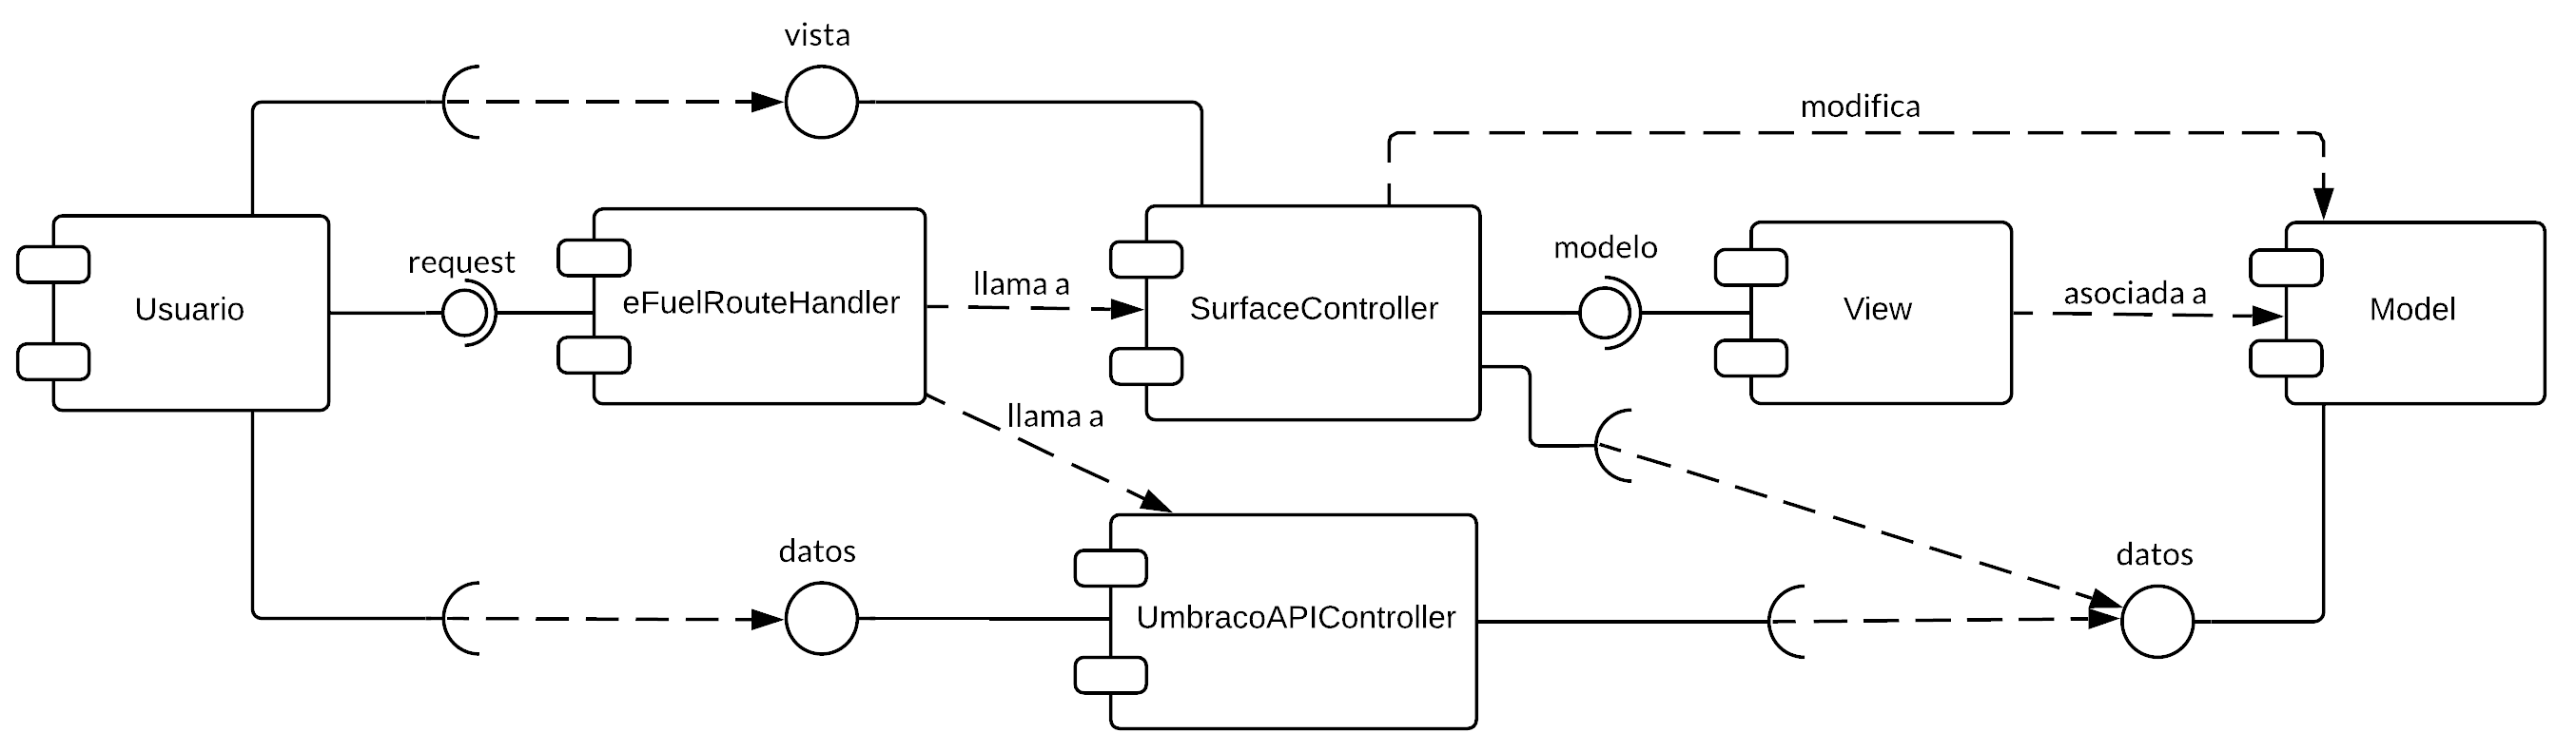
\includegraphics[width=\textwidth]{component_diagram.png}
    \caption{Diagrama de Componentes}
    \label{fig:component_diagram}
    \centering
\end{figure}

\subsection{Organización del proyecto}
El proyecto está compuesto por 3 módulos:

\begin{itemize}
    \item \verb|EF_API|: contiene los controladores usados para implementar los servicios web. Estos controladores heredan de la clase \verb|UmbracoApiController| y su función es buscar datos (normalmente listas) y devolverlos en formato JSON al cliente. Se creó un controlador por cada entidad principal del sistema (clientes, transportes, órdenes, etc).
    \item \verb|EF_Core|: contiene los controladores del patrón MVC, los manejadores de rutas (Route Handlers) para estos y los modelos que sirven para interactuar con la base de datos. Los controladores de este módulo heredan de la clase \verb|SurfaceController| y su función es, básicamente, buscar datos y devolver vistas. Hay un controlador por cada tipo de entidad principal del sistema (clientes, transportes, órdenes, etc).
    \item \verb|EF_Miscelaneous|: contiene todos los archivos de la Vista del patrón MVC, esto es, las vistas (HTML), los archivos de estilo (CSS) y los scripts del front end (JavaScript). Además contiene los archivos de configuración de Fluidity (ver sección \ref{umbracoComponents}).
\end{itemize}

A continuación se muestran los diagramas de clases de \verb|EF_API| y \verb|EF_Core|. Luego se mostrará una lista con las vistas en \verb|EF_Miscelaneous|.

\begin{figure}[H]
    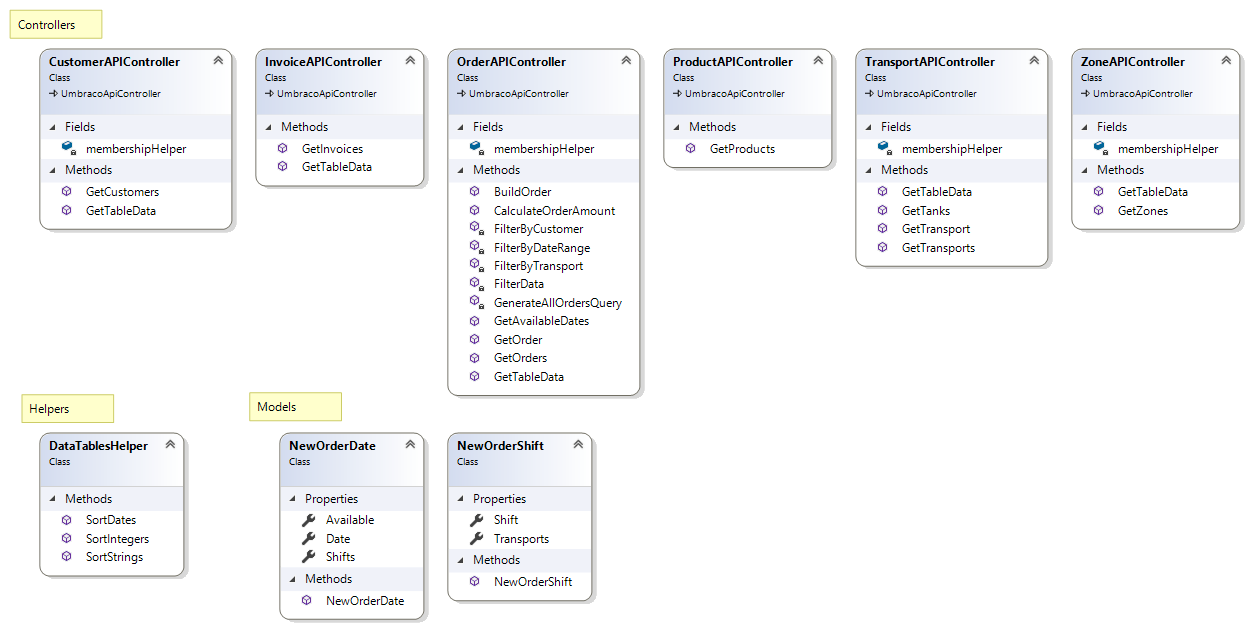
\includegraphics[width=\textwidth]{EF_API_class_diagram.png}
    \caption{Diagrama de Clases (EF\_API)}
    \label{fig:EF_API_class_diagram}
    \centering
\end{figure}

\begin{figure}[H]
    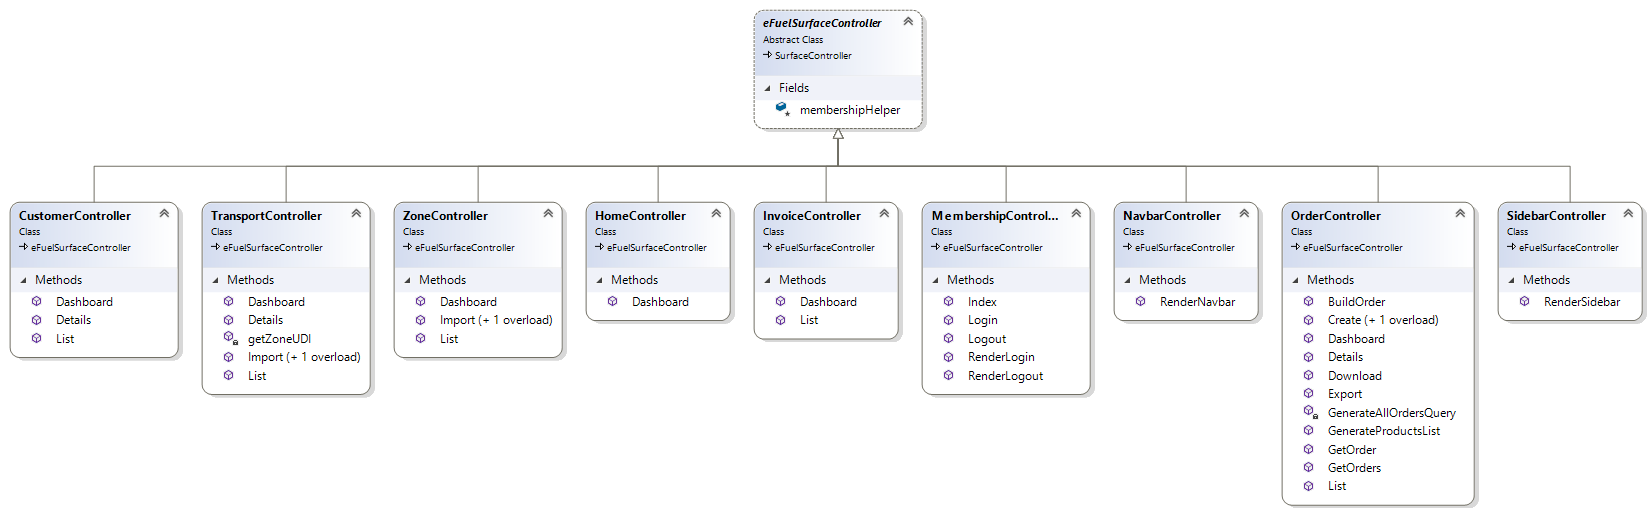
\includegraphics[width=\textwidth]{EF_Core_class_diagram_controllers.png}
    \caption{Diagrama de Clases (EF\_Core/Controllers)}
    \label{fig:EF_Core_class_diagram_controllers}
    \centering
\end{figure}

\begin{figure}[H]
    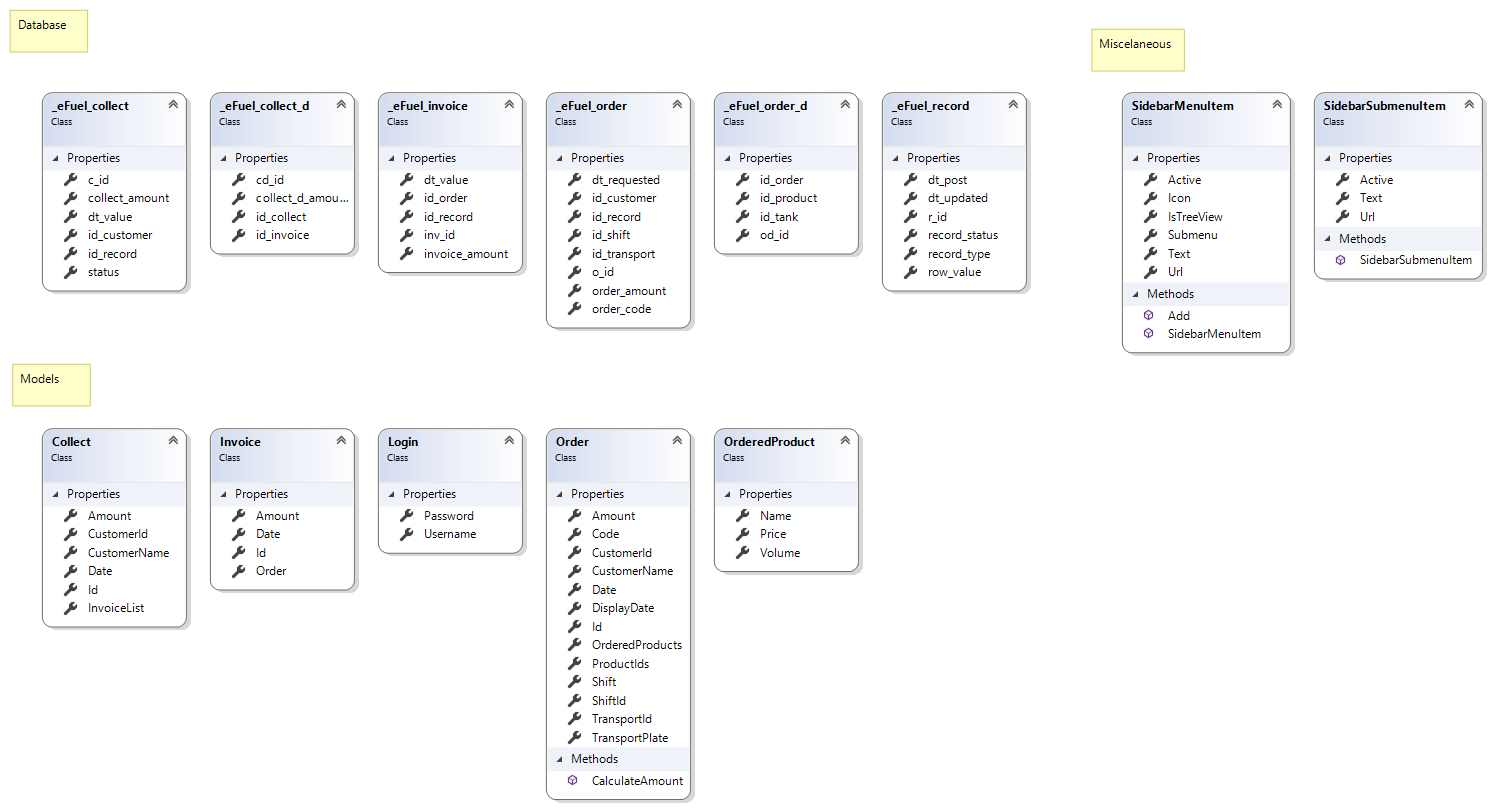
\includegraphics[width=\textwidth]{EF_Core_class_diagram_models.png}
    \caption{Diagrama de Clases (EF\_Core/Models)}
    \label{fig:EF_Core_class_diagram_models}
    \centering
\end{figure}

\begin{figure}[H]
    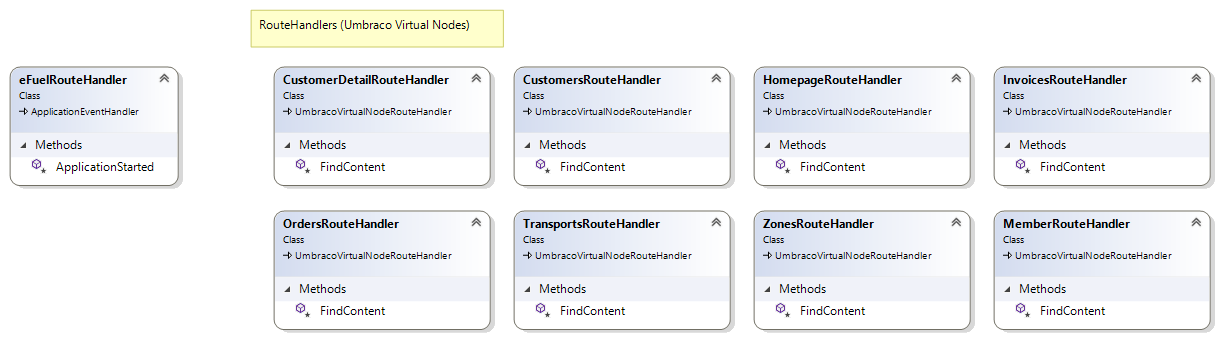
\includegraphics[width=\textwidth]{EF_Core_class_diagram_routing.png}
    \caption{Diagrama de Clases (EF\_Core/Routing)}
    \label{fig:EF_Core_class_diagram_routing}
    \centering
\end{figure}

\subsubsection{Vistas del sistema}
A continuación una lista de las vistas organizadas por carpetas. Hay una carpeta para cada \verb|SurfaceController| (ver figura \ref{fig:EF_Core_class_diagram_controllers}) además de una carpeta (\verb|Shared|) que contiene las vistas usadas por uno o más controladores (en su mayoría son Partial Views). Cada carpeta puede considerarse como el Modelo al que están asociadas cada una de las vistas dentro de ella, por esta razón nombraremos la primera columna "Modelos" ya que ayuda a entender la estructura del sistema desde el punto de vista de MVC.

\begin{longtable}{ | p{5.5em} | p{7em} | p{15em} | c | }
    \hline
    \rowcolor{gray!30}
    \multicolumn{1}{|c|}{Modelo} &
    \multicolumn{1}{|c|}{Nombre} &
    \multicolumn{1}{|c|}{Descripción} &
    \multicolumn{1}{|c|}{Partial View} \\
    \hhline{====}
    \endhead

    \hline
    \endfoot

    \endlastfoot

    Customer
        & Dashboard & Panel con las acciones principales que se pueden realizar sobre los clientes & - \\
    \cline{2-4}
        & Details & Información detallada de un cliente & - \\
    \cline{2-4}
        & Edit & Formulario para editar la información de un cliente & \checkmark \\
    \cline{2-4}
        & List & Tabla con todos los clientes que puede ver el usuario & \checkmark \\
    \hline

    Home
        & Dashboard & Mensaje de bienvenida (eventualmente debe mostrar las opciones más importantes del sistema) & - \\
    \hline

    Invoice
        & Dashboard & Panel con las acciones principales que se pueden realizar sobre las facturas & - \\
    \cline{2-4}
        & List & Tabla con las facturas & \checkmark \\
    \hline

    Membership
        & Index & Página de inicio de sesión & - \\
    \hline

    Order
        & Create & Formulario para crear un nuevo pedido & \checkmark \\
    \cline{2-4}
        & Dashboard & Panel con las acciones principales que se pueden realizar sobre los pedidos & - \\
    \cline{2-4}
        & Details & Información detallada de un pedido & - \\
    \cline{2-4}
        & List & Tabla con todos los pedidos que puede ver el usuario junto con los filtros y opciones de exportar la lista, crear un nuevo pedido y filtrar la lista de pedidos & \checkmark \\
    \hline

    Shared
        & AppTitle & Título de la página actual & \checkmark \\
    \cline{2-4}
        & Breadcrumbs & Cadena de enlaces a las páginas superiores a la página actual & \checkmark \\
    \cline{2-4}
        & LoginForm & Formulario de inicio de sesión & \checkmark \\
    \cline{2-4}
        & LogoutButton & Botón de cerrar sesión & \checkmark \\
    \cline{2-4}
        & Master & Estructura del sitio que es común a todas las páginas del sitio (excepto la página de inicio de sesión). Barra de navegación, barra lateral, título, etc. & - \\
    \cline{2-4}
        & Navbar & Barra de navegación superior & \checkmark \\
    \cline{2-4}
        & Sidebar & Barra de navegación lateral, contiene las secciones del sitio & \checkmark \\
    \hline

    Transport
        & Dashboard & Panel con las acciones principales que se pueden realizar sobre los transportes & - \\
    \cline{2-4}
        & Details & Información detallada de un transporte & - \\
    \cline{2-4}
        & Import & Formulario para importar una lista transportes & \checkmark \\
    \cline{2-4}
        & List & Tabla con los transportes que puede ver el usuario & \checkmark \\
    \hline

    Zone
        & Dashboard & Panel con las acciones principales que se pueden realizar sobre las zonas & - \\
    \cline{2-4}
        & Import & Formulario para importar una lista zonas & \checkmark \\
    \cline{2-4}
        & List & Tabla con las zonas que puede ver el usuario & \checkmark \\
    \hline

    \caption{Vistas del front end}
    \label{table:vistas}
\end{longtable}

\subsection{Componentes de Umbraco}
\subsubsection{Datatypes}

\begin{longtable}{  l | l  }
    \hline\hline
    \rowcolor{gray!30}
    \textbf{Datatype} & \textbf{Uso} \\
    \hline\hline
    \endhead

    \hline
    \endfoot

    \endlastfoot

    Collect picker & Seleccionar un cobro \\
    Customer picker & Seleccionar un cliente \\
    Invoice picker & Seleccionar una factura \\
    Order picker & Seleccionar un pedido \\
    Product picker & Seleccionar un producto \\
    Shift picker & Seleccionar un turno \\
    Tank picker & Seleccionar un tanque \\
    Transport picker & Seleccionar un transporte del árbol de contenido \\
    Customer node picker & Seleccionar el nodo de un cliente del árbol de contenido \\
    Zone node picker & Seleccionar el nodo de una zona del árbol de contenido \\
    Attached images & Seleccionar una imagen \\
    Customer status & Elegir uno de los estados del cliente \\
    EAN-UPC & Introducir el código EAN o UPC de un producto \\
    Email address & Introducir un correo electrónico \\
    On Off & Elegir uno de 2 estados: on u off \\
    Payment terms & ELegir una forma de pago \\
    Tank list & Agregar o eliminar tanques a un transporte \\
    Textstring max65 & Introducir texto de máximo 65 caracteres \\
    Transport status & Seleccionar el estado de un transporte \\

    \hline

    \caption{Datatypes}
    \label{table:datatypes}
\end{longtable}

Todos los Datatypes creados para eFuel tienen el prefijo \emph{\_eFuel::} en su nombre.

\subsubsection{Doctypes}
El árbol de contenidos de eFuel se muestra en la figura \ref{fig:content_tree}. Luego se describen los Doctypes de la aplicación.

\begin{figure}[h]
    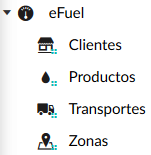
\includegraphics[width=0.3\textwidth, center]{content_tree.png}
    \caption{Árbol de contenido de eFuel}
    \label{fig:content_tree}
    \centering
\end{figure}

\begin{longtable}{ | p{5em} | l | l | }
    \hline
    \rowcolor{gray!30}
    \multicolumn{1}{|c|}{Doctype} &
    \multicolumn{1}{|c|}{Propiedades} &
    \multicolumn{1}{|c|}{Datatype} \\
    \hline
    \endhead

    \hline
    \endfoot

    \endlastfoot

    Cliente
        & Descripción & Textarea \\
        \cline{2-3}
        & Código de impuestos & Textstring \\
        \cline{2-3}
        & Estado & Customer status \\
        \cline{2-3}
        & Zona & Zone node picker \\
        \cline{2-3}
        & Forma de pago & Payment terms \\
        \cline{2-3}
        & Ok days & Numeric \\
        \cline{2-3}
        & Due days & Numeric \\
        \cline{2-3}
        & Dirección & Textstring \\
        \cline{2-3}
        & Teléfono & Textstring \\
        \cline{2-3}
        & Correo & Email address \\
        \cline{2-3}
        & Contacto & Textstring \\
        \cline{2-3}
        & Código ERP & Textstring \\
        \cline{2-3}
        & Código externo & Textstring \\
        \cline{2-3}
        & Imagen & Attached images \\
    \hline

    Producto
        & Precio base & Decimal \\
        \cline{2-3}
        & Descripción & Textarea \\
        \cline{2-3}
        & Código ERP & Textstring \\
        \cline{2-3}
        & Código externo & Textstring \\
        \cline{2-3}
        & SKU & Textstring \\
        \cline{2-3}
        & EAN/UPC & EAN-UPC \\
        \cline{2-3}
        & Imagen & Attached images \\
    \hline

    Tanque
        & Volumen & Numeric \\
    \hline

    Transporte
        & Placa chuto & Textstring \\
        \cline{2-3}
        & Placa cisterna & Textstring \\
        \cline{2-3}
        & Zona & Zone node picker \\
        \cline{2-3}
        & Nombre del conductor & Textstring \\
        \cline{2-3}
        & Volumen total & Numeric \\
        \cline{2-3}
        & Estado & Transport status \\
        \cline{2-3}
        & Tanques & Tank list \\
        \cline{2-3}
        & Código ERP & Textstring \\
        \cline{2-3}
        & Código externo & Textstring \\
        \cline{2-3}
        & Imagen & Attached images \\
    \hline

    Turno
        & Descripción & Textstring \\
        \cline{2-3}
        & Código ERP & Textstring \\
        \cline{2-3}
        & Código externo & Textstring \\
    \hline

    Zona
        & Código ERP & Textstring \\
        \cline{2-3}
        & Código externo & Textstring \\
    \hline

    \caption{Doctypes}
    \label{table:doctypes}
\end{longtable}